\section{Objetivos}
O presente trabalho tem por objetivo construir uma curva de EFV (do
ingês, \emph{equilibrium flash vaporization}) para um petróleo qualquer. A
composição do óleo será determinada a partir de valores de TBP (do ingês,
\emph{true boiling point} - ponto de ebulição verdadeiro) obtidos de
informações fornecidadas pelo site da \citeauthor{TOTSA2016}.

Para isso, inicialmente será realizada uma breve contextualização de alguns
tópicos, tais como análises de TBP e EFV, bem como algumas regras de mistura
que serão usadas no trabalho.

\section{Introdução teórica}

\subsection{TBP}
A curva de TBP (\emph{true boiling point}) ou PEV (ponto de ebulição verdadeiro)
é um gráfico que contem os valores dos pontos de ebulição  dos componentes quase puros q
ue estão contidos em um petróleo bruto ou em alguma de suas frações. Antigamente, 
essa curva era construída em laboratório utilizando equipamentos complexos de 
destilação em batelada com cem ou mais estágios de equilíbrio e alta razão de 
refluxo. Hoje em dia, esse mesmo gráfico é feito por meio de espectroscopia de massa, 
muito mais rápida e com precisão mais elevada \cite{Jones2006}.

\subsection{EFV}


A curva EFV (\emph{equilibrium flash vaporization}) fornece a informação da
temperatura que um dado volume de destilado será vaporizado. Esse vapor
destilado está sempre em equilíbrio com a fase líquida e os ensaios de EFV são
sempre conduzidos em pressão atmosférica. De acordo com \citeonline{Eckert2008},
esse ensaio é raramente realizado, pois é muito trabalhoso. Em uma série de
experimentos, são medidas as temperaturas de equilíbrio para diferentes valores especificados de 
 fração de líquidos. Esse tipo de ensaio também é usado para projetar processos
 onde ocorre equilíbrio líquido-vapor como, por exemplo, refervedores, condesadores
  parciais, etc).
  
\subsection{Equação de Estados: Peng-Robinson}

 A equação de \citeonline{Peng1976}, apresentada na
 \autoref{eq:PReq}, faz o uso do fator acêntrico de Pitzer ($w$). Com esse 
 parâmetro, espera-se que esse modelo seja melhor aplicado para diferentes classes
 de moléculas \cite{Koretsky2013}.
      
\begin{equation}\label{eq:PReq}
P = \frac{RT}{v - b} - \frac{\alpha T(r)}{v(v+b)+b(v-b)}
\end{equation} 

O valor de $\alpha T(r)$ é descrito na \autoref{eq:alfa}:
 \begin{equation}\label{eq:alfa}
\alpha T(r) = [1 +
 \kappa(1-\sqrt{T_r})]^2
\end{equation} 
onde $\kappa = (0,37464+1,54226w-0,26992w^2)$. 
 O fator acêntrico de Pitzer caracateriza o quão ``não-esférica'' é a molécula,
 assim, pode ser atribuída para uma classe de substâncias com
 características semelhantes. A \autoref{eq:w} apresenta a definição desse fator
 acêntrico:
 
  \begin{equation}\label{eq:w}
w \equiv -1 - log_{10}\left [ P^{sat} \frac{( T_r = 0,7 )}{P_c}
\right ]
\end{equation} 
onde $ P^{sat} \left ( T_r = 0,7 \right )$ é a pressão de saturação de dada
substância em uma termperatura reduzida igual a 0,70.

\subsection{Regras de Mistura}

\citeonline{Koretsky2013} afirma que a abordagem mais prática no uso de equações de estado
é utilizar regras de mistura que se baseiam nos dados dos componentes puros e 
aplicam tais para os tipos de interações presentes na mistura em questão. A 
\autoref{eq:aij} apresenta a formulação para o termo relacionado à força de
atração entre duas moléculas diferentes em uma mistura.

\begin{equation}\label{eq:aij}
a_{mix} = \sum_i\sum_jy_iy_ja_{ij}
\end{equation}
onde $y$ são as frações molares dos componentes $i$ e $j$ e $a_{ij}$ é a
atração entre as molecúlas dos mesmos componentes $i$ e $j$. O termo de atração
da \autoref{eq:aij} segue as premissas apresentadas a seguir, nas Equações
\ref{eq:aij2}, \ref{eq:aij3} e \ref{eq:aij4}. 

\begin{equation}\label{eq:aij2}
a_{ij} = a_{ji}
\end{equation}

\begin{equation}\label{eq:aij3}
a_{ij} = \sqrt{a_ia_j}(1 - k_{ij})
\end{equation}

\begin{equation}\label{eq:aij4}
a_{i} = a_{ii}
\end{equation}

A \autoref{eq:bmix} apresenta a expressão para o termo relacionado ao volume
excluído quando ocorre a mistura.

\begin{equation}\label{eq:bmix}
b_{mix} = \sum_iy_ib_i
\end{equation}

\subsubsection{van der Waals (vdW)}
\citeonline{Kwak1986} mostra que, para uma mistura binária cuaj energia potencial
intermolecular expressa na \autoref{eq:uij}, as regras de mistura derivadas são 
as Equações \ref{eq:sigmacubo} e \ref{eq:esigmacubo}.

\begin{equation}\label{eq:uij}
u_{ij}(r) = \epsilon_{ij}f(r/\sigma_{ij})
\end{equation}

\begin{equation}\label{eq:sigmacubo}
\sigma^3 = \sum_i^n\sum_j^nx_ix_j\sigma_{ij}^3
\end{equation}

\begin{equation}\label{eq:esigmacubo}
\varepsilon\sigma^3 = \sum_i^n\sum_j^nx_ix_j\varepsilon_{ij}\sigma_{ij}^3
\end{equation}
onde $\varepsilon_{ij}$ é o parâmetro de interação energética entre as moléculas
$i$ e $j$, e $\sigma_{ij}$ é a distância de interação intermolecular entre duas
moléculas. Os coeficientes $a$ e $b$ da equação de estado de van der Waals são
proporcionais aos valores de $\varepsilon$ e $\sigma$.

Sabendo que $\sigma_{ij}$, para $i \neq j$, a interação entre diâmetro
distintos, para moléculas esféricas, é mostrado na \autoref{eq:sigmaij}:

\begin{equation}\label{eq:sigmaij}
\sigma_{ij} = \frac{\sigma_{ii} + \sigma_{jj}}{2}
\end{equation}

Tal leva a seguinte expressão de $b_{ij}$ para moléculas esféricas, conforme
\autoref{eq:bij}:

\begin{equation}\label{eq:bij}
b_{ij} = \left ( \frac{b_{ii}^{1/3} + b_{jj}^{1/3}}{2} \right )^3
\end{equation}

E, para moléculas não esféricas, a relação é descrita na \autoref{eq:bij2}:

\begin{equation}\label{eq:bij2}
b_{ij} = (1 - l_{ij})\left [ b_{ii}^{1/3} + b_{jj}^{1/3} \right ]^3
\end{equation}

\subsubsection{Regra de Mistura vdW para EoS PR}

A equação de Peng-Robinson (\autoref{eq:PReq}) pode ser reescrita como mostrado
na \autoref{eq:PRnew}:

\begin{equation}\label{eq:PRnew}
Z = \frac{\nu}{\nu - b} - \frac{(a/RT) + d - 2 \sqrt{ad/RT}}{(\nu + b) +
(b/\nu)(\nu - b)}
\end{equation}
onde: $a = a(T_c)(1 + \kappa)^2$ e $d = a(T_c)\kappa^2/RT_c$.

Assim, a equação de estado de Peng-Robinson apresenta 3 termos
independentes: $a$, $b$ e $d$. Deste modo, seguindo o modelo antes mostrado para
regras de mistura de van der Waals, tem-se:

\begin{equation}\label{eq:PRnew1}
a = \displaystyle\sum_i^n\sum_j^nx_ix_ja_{ij}
\end{equation}
\begin{equation}\label{eq:PRnew2}
b = \displaystyle\sum_i^n\sum_j^nx_ix_jb_{ij}
\end{equation}
\begin{equation}\label{eq:PRnew3}
d = \displaystyle\sum_i^n\sum_j^nx_ix_jd_{ij}
\end{equation}
onde: 
\begin{equation}\label{eq:PRnew4}
a_{ij} = (1 - k_{ij})\sqrt{a_{ii}a_{jj}}
\end{equation}
\begin{equation}\label{eq:PRnew5}
b_{ij} = (1 - l_{ij})\left [ \frac{b_{ii}^{1/3} + b_{jj}^{1/3}}{2} \right]^3
\end{equation}
\begin{equation}\label{eq:PRnew6}
d_{ij} = (1 -m_{ij})\left [ \frac{d_{ii}^{1/3} + d_{jj}^{1/3}}{2} \right]^3
\end{equation}
\subsubsection{SCMR}
Conforme é apresentado por \citeonline{Staudt2012}, esta regra de
mistura apresenta volume de excesso negligenciável e a fração $ u =
\frac{V}{b} $ é constante. A \autoref{eq:gphi1} apresenta a expressão para 
energia de Gibbs em excesso e a \autoref{eq:lnphi} para o coeficiente de
fugacidade para mistura.

\begin{equation}\label{eq:gphi1}
\frac{G_\phi^E}{RT} = ln\phi - \sum_ix_iln\phi_i
\end{equation}

\begin{equation}\label{eq:lnphi}
ln\phi = (Z - 1) - ln(Z - \beta) + qI
\end{equation}

Utilizando a definição de volume em excesso ($V^E$) e abrindo o termo $ln(Z -
\beta)$, obtem-se a \autoref{eq:gphi2}:

\begin{equation}\label{eq:gphi2}
\frac{G_\phi^E}{RT} = \frac{PV^E}{RT} + \sum_ix_iln\left ( \frac{V_i - b_i}{V -
b} \right ) + qI - \sum_ix_iq_iI_i
\end{equation}

Assumindo que o volume em excesso é negligenciável, obtem-se a
\autoref{eq:gphi3}:

\begin{equation}\label{eq:gphi3}
\frac{G_\phi^E}{RT} = \sum_ix_iln\left ( \frac{V_i - b_i}{V^{Id} -
b} \right ) + qI^{Id} - \sum_ix_iq_iI_i
\end{equation}
onde $b$ é calculado via \autoref{eq:bmix}, o volume das substâncias puras
$V_i$, bem como $I^{Id}$ e $I_i$, devem ser calculados utilizando a raiz do tipo
líquido do sistema puro nas temperaturas e pressões do sistema. Para baixas pressões, pode-se igualar os
 modelos de Gibbs em excesso para a fugacidade e o coeficiente de atividade
 ($G_\phi^E$ = $G_\gamma^E$).

\subsubsection{PSRK}

No trabalho de \citeonline{Chen2002}, é mostrado como é obtido o parâmetro $a$.
A expressão para tal é ilustrada na \autoref{eq:abrt}:


\begin{equation}\label{eq:abrt}
\frac{a}{bRT} = \sum x_i\frac{a_{ii}}{b_iRT}+\frac{1}{A}\left (
\frac{g_0^E}{RT}+\sum x_iln\frac{b}{b_i} \right )
\end{equation}
onde $A$ foi setado como -0,64663. \citeonline{Fischer1996} afirmam
que PSRK gera bons resultados para as propriedades termodinâmicas, especialmente para 
equilíbrios líquido-vapor em altas pressões.

\subsection{Modelo de Atividade: Scatchard-Hildebrand}
Segundo \citeonline {Brignole2013}, a teoria de soluções regulares de
Scatchard-Hildebrand provém do modelo de Flory-Huggins considerando que a entropia da mistura corresponde ao valor 
de uma mistura ideal. Além disso, ela leva em consideração a existência do 
calor da mistura que ocorre devido às interações energéticas moleculares. 
Uma vez que todas as combinações em uma mistura binária sejam levadas em 
conta, a expressão para o coeficiente de atividade do componente 1 é
apresentada na \autoref{eq:lngamma1}:

\begin{equation}\label{eq:lngamma1}
ln\gamma_1 = \frac{\nu_1\varphi_2^2(\delta_1-\delta_2)^2}{RT}
\end{equation}
onde $\gamma_1$é o coeficiente de atividade e $\nu_1$ é o volume molar para o
componente 1 e $\varphi_2$ é a fração volumétrica do componente 2. Os parâmetros
de solubilidade dos componentes puros ($\delta_1$ e $\delta_2$) podem ser
obtidos a partir da energia interna de vaporização de cada componente puro $i$
($\Delta u_i^v$), como um líquido saturado na temperatura do sistema
(\autoref{eq:deltai}):

\begin{equation}\label{eq:deltai}
\delta_i = \left ( \frac{\Delta u_i^V}{\nu_i^L} \right )^{\frac{1}{2}}
\end{equation}

O termo entre parânteses da \autoref{eq:deltai} é denominado de densidade de energia
coesiva e o parâmetro de solubilidade para misturas multicomponentes é mostrada
na \autoref{eq:delta}:

\begin{equation}\label{eq:delta}
\delta = \sum_i\sum_j\phi_i\phi_j\delta_{ij}^2
\end{equation}

onde

\begin{equation}\label{eq:deltaij}
\delta_{ij}^2 = \delta_1\delta_j
\end{equation}

Assim, substituindo a \autoref{eq:deltaij} na \autoref{eq:delta}, pode-se obter
uma nova expressão $\delta$, como é mostrado na \autoref{eq:delta2}.

\begin{equation}\label{eq:delta2}
\delta = \sum_i\phi_i\delta_i
\end{equation}


\section{Metodologia}

\subsection{Dados experimentais}

Para a realização do trabaho, foram utilizados dados de análise de um
petróleo do poço CLOV localizado na Angola. Essa informação foi
coletada no site da \emph{Total Oil Trading S.A.} (\citeauthor{TOTSA2016}). O
principal fator para a escolha desse poço foi que a última análise do óleo foi
realizada recentemente, em janeiro de 2016. Os resultados das análises
físico-químicas do pretróleo, bem como os dados de Pronto de Ebulição Verdadeiro
(PEV ou TBP) estão mostrados nas Tabelas \ref{tab:dados} e \ref{tab:tbp}.

\begin{table}[htb]
\renewcommand{\arraystretch}{1.3}
\caption{Característica do petróleo extraído do poço CLOV - Angola}
\footnotesize 
\center
\begin{tabular}{llc}
\toprule
 {Data da análise}						&						&	{25/01/20016}	\\
 {Densidade a 15$^\circ$C (kg/m$^3$)}	&						&	{858,9}			\\
 {$^\circ$API}							&						&	{33,2}			\\
 {Bbl/mt}								&						&	{7,336}			\\
 {Acidez (mg KOH/g)}					&						&	{0,54}			\\
 {Enxofre (massa\%)}					&						&	{0,249}			\\
 {Sulfeto de Hidrogênio (mg/kg)}		&						&	{1}				\\
 {Enxofre de mercaptanos (mg/kg)}		&						&	{3}				\\
 {Viscosidade (cSt)} 					&		{10 $^\circ$C}	&	{19,3}			\\
 { }				 					&		{50 $^\circ$C}	&	{5,4}			\\
 {Ponto de Fluidez ($^\circ$C)}			&						&	{-6}			\\
 {Nitrogênio total (massa\%)}			&						&	{0,142}			\\
 {Cera (massa\%)}						&						&	{-}				\\
 {Temp. aparente de cera  ($^\circ$C)}	&						&	{-}				\\
 {RVP a 37,8 $^\circ$C (kPa)}			&						&	{26}			\\
 {Umidade (vol\%)}						&						&	{-}				\\
 {NaCl (mg/kg)}							&						&	{-}				\\
 {Níquel (mg/kg)}						&						&	{7,7}			\\
 {Vanádio (mg/kg)}						&						&	{1,9}			\\
 {Ferro (mg/kg)}						&						&	{-}				\\
 {Mercúrio ($\mu$g/kg)}					&						&	{-}				\\
 {Leves (vol\%)}						&	{Etano}				&	{0,06}			\\
 										&	{Propano}			&	{0,57}			\\
 										&	\emph{iso}-Butano	&	{0,33}			\\
 										&	\emph{n}-Butano		&	{0,94}			\\
\bottomrule
\multicolumn{3}{c}{Fonte: \citeonline{TOTSA2016}}
\end{tabular}
\label{tab:dados}
\end{table}
\clearpage

\begin{table}[htb]
\renewcommand{\arraystretch}{1.3}
\caption{Dados de Ponto de Ebulição Verdadeiro (PEV ou TBP)
para o poço CLOV - Angola}
\sisetup{table-format=2.2,round-mode=places,round-precision=2}
\footnotesize
\center
\begin{tabular}{S[table-format=3.0,round-mode=places,round-precision=0]SS|S[table-format=3.0,round-mode=places,round-precision=0]SS}
\toprule
   {T} & {\%. vap.} & {\% vap.}&{T} &
   {\% vap.} & {\% vap.}\\
   {($^\circ$C)} & {(massa)} & {(vol.)}&{($^\circ$C)} &
   {(massa)} & {(vol.)}\\
\midrule 
80  &4.88  &6.60&  340 & 49.61 &53.57\\
90  &5.83  &7.73&  360 & 53.30 &57.18\\
100 &7.01  &9.10&  380 & 56.86 &60.64\\
120 &10.02 &12.54& 400 & 60.31 &63.96\\
140 &13.62 &16.56& 420 & 63.66 &67.16\\
160 &17.05 &20.31& 440 & 66.91 &70.25\\
180 &19.98 &23.47& 460 & 70.06 &73.22\\
200 &22.86 &26.52& 480 & 73.09 &76.05\\
220 &26.08 &29.90& 500 & 75.99 &78.75\\
240 &29.72 &33.65& 520 & 78.73 &81.28\\
260 &33.64 &37.67& 540 & 81.30 &83.64\\
280 &37.71 &41.78& 560 & 83.68 &85.81\\
300 &41.78 &45.85& 580 & 85.87 &87.80\\
320 &45.76 &49.80&     &       &     \\
\bottomrule
\multicolumn{6}{c}{Fonte: \citeonline{TOTSA2016}}
\end{tabular}
\label{tab:tbp}
\end{table}

\subsection{Procedimento de Cálculo}
Para a obtenção da curva EFV, foram utilizados os dados experimentais
de TBP e fez-se o uso do simulador de processo $iiSE$. O modelo termodiâmico
utilizado foi o de Peng-Robinson com três diferentes regras de mistura: van der
Waals (vdW), PSRK e SCMR. Para as duas últmas, é necessário o uso de um modelo
de Gibbs em excesso ($g^E$), portanto utilizou-se para ambas o modelo de
Scatchard-Hildebrand.

Para a configuração do petróleo no $iiSE$, foram inseridos os valores dos
percentuais volumétricos dos quatro leves contidos nos resultados da análise experimental e
foi feito um corte em 30 pseudos. Para a avaliação da composição do líquido e do
vapor em função do percentual vaporizado, utilizou-se apenas as frações dos
leves e de 6 pseudos com massas molares distintas, os quais foram escolhidos
aleatoriamente.

\clearpage 

\section{Resultados}

\subsection{Análise das curvas TBP e EFV} 

Realizou-se a simulação da curva de EFV no \emph{software} $iiSE$, para todas as
regras de misturas, variando-se a temperatura de 0,0 $^\circ$C até 600,0
$^\circ$C, com passo de $\Delta$T unitário. Deste modo, foram obtidos 600 pontos
para cada simulação, com o intuito de, além de construir a curva EFV, poder
fazer uma comparação entre cada teste.

Primeiramente, buscou-se conhecer qual foi a temperatura onde iniciou-se a
vaporização do componente mais leve e o instante onde ocorre a vaporização do
mais pesado. Contudo, observa-se que, nas condições utilizadas no presente
trabalho, o simulador apresentou dificuldade na predição dos valores quando a
vaporização aproximou-se de 90,5{\%}. Deste modo, considerou-se, então, que a
temperatura final a ser comparada seria exatamente a anterior àquela que o
simulador não foi capaz de predizer corretamente. A \autoref{tab:result1}
apresenta os valores de temperatura (inicial e final da vaporização), bem como o
passo de $\Delta$T.

\begin{table}[htb]
\renewcommand{\arraystretch}{1.3}
\caption{Temperaturas, iniciais e finais, e passos de T para cada regra de
mistura na simulação EFV para o óleo CLOV - Angola}
\sisetup{table-format=2.2,round-mode=places,round-precision=2}
\footnotesize
\center 
\begin{tabular}{lccc}   
\toprule
   &{Temperatura Inicial}&{Temperatura Final}&\multirow{2}{*}{$\Delta$T} \\
  &{da Fração Vaporizada ($^\circ$C)}&{da Fração Vaporizada
   ($^\circ$C)} & \\
\midrule 
{EFV: PR+SCMR}	&	73	&	472		&	1 \\
{EFV: PR+VDW}	&	75	&	468		&	1 \\
{EFV: PR+PSRK}	&	51	&	469		&	1 \\
\bottomrule
%\multicolumn{4}{c}{Fonte: \citeonline{TOTSA2016}}
\end{tabular}
\label{tab:result1}
\end{table}

A \autoref{fig:efv} apresenta os resultados simulados para as curvas EFV
utilizando a equação de estado Peng-Robinson com as diferentes regras de
mistura. Além disso, está graficada a curva TBP do óleo, cujos dados foram
obtidos do laudo de análise do mesmo.
\clearpage

\begin{figure}[htb]
\centering
{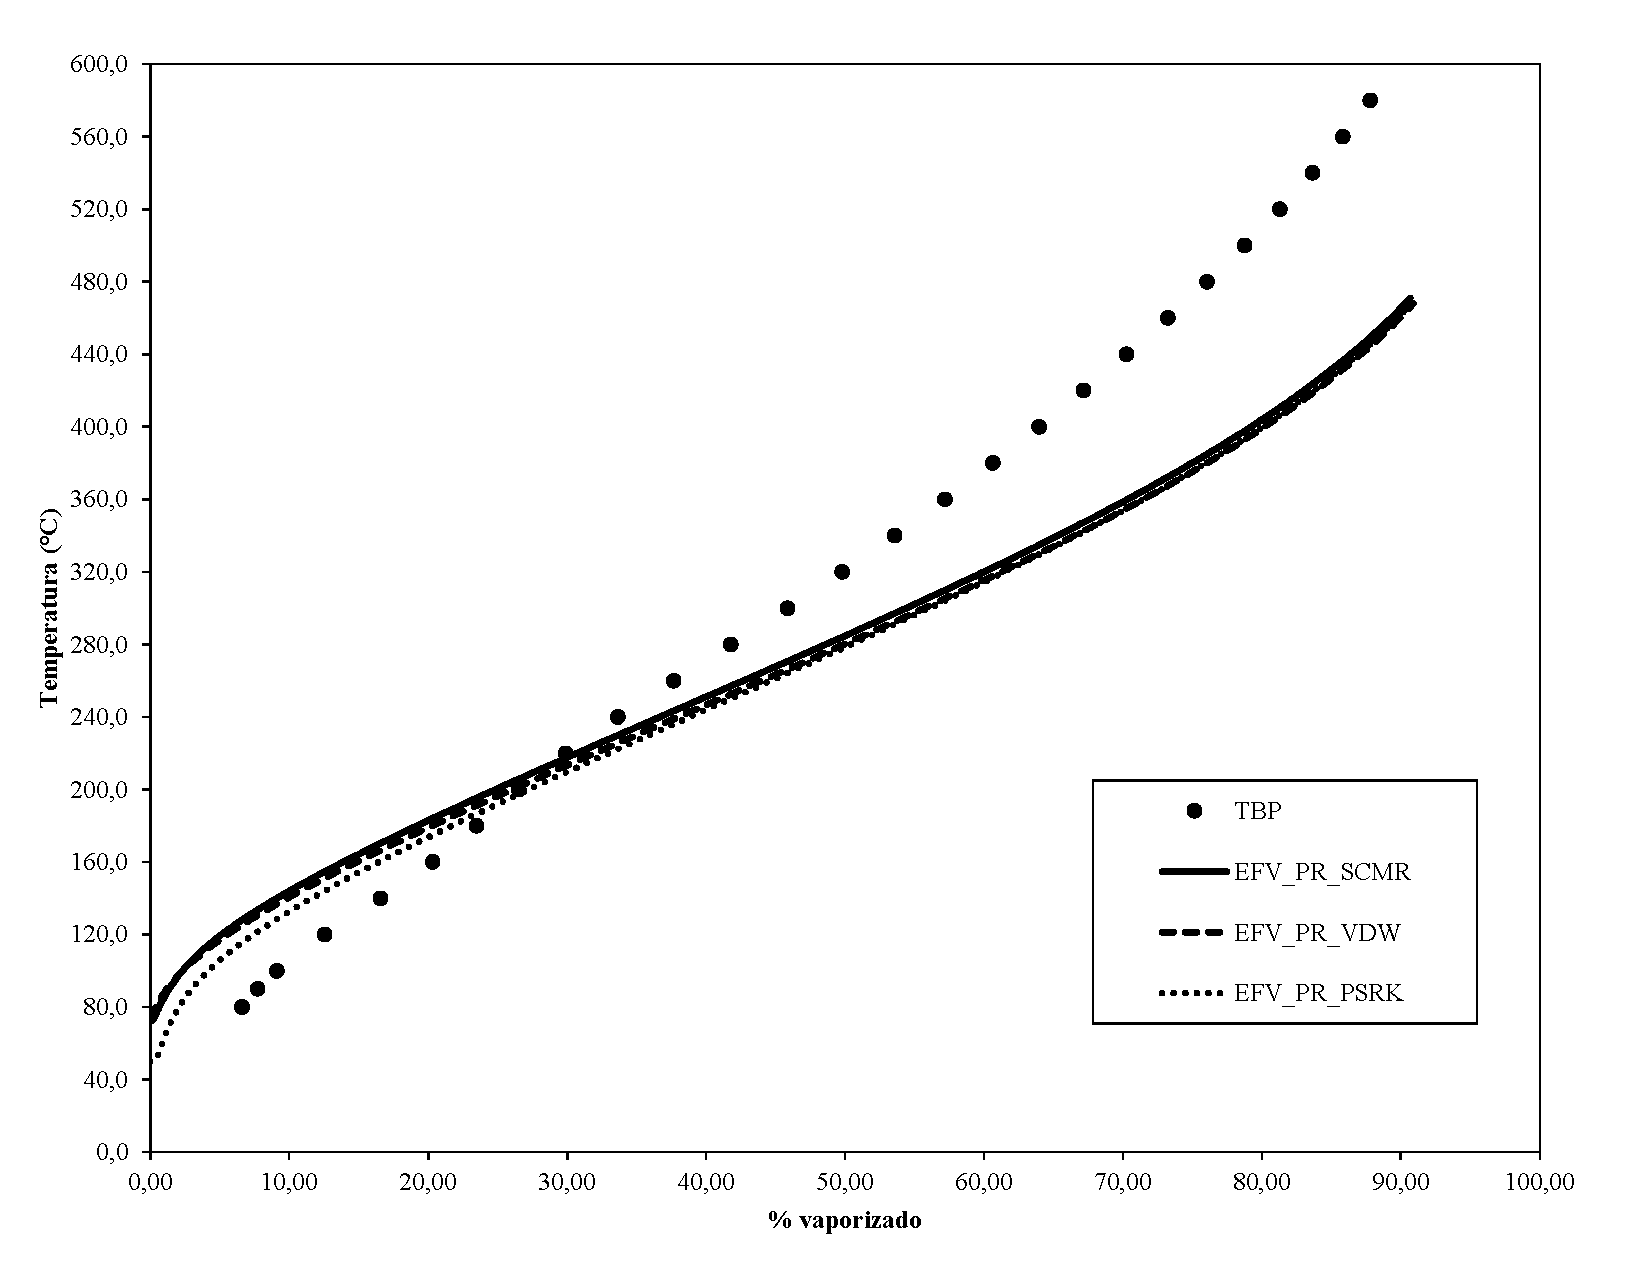
\includegraphics[width=1.0\textwidth]{img/trab3.pdf}} 
\caption{Curva de TBP e EFV para o petróleo do poço CLOV - Angola}
\label{fig:efv}
\end{figure} 


Ao analisar a \autoref{fig:efv}, nota-se que as curvas EFV com as regras de
mistura SCRM e vdW apresentaram comportamentos semelhantes. Contudo, ao
utilizar-se PSRK (\emph{Predictive Soave-Redlich-Kwong}), observa-se um desvio
considerável nos valores iniciais, quando comparado às outras duas. Este fato pode ser explicado devido à não utilização
do ``pacote fechado'' desta regra de mistura, uma vez que para o modelo de Gibbs
em excesso foi utilizado Scatchard-Hildebrand ao invés do UNIFAC(PSRK). Além
disso, a equação de estado a ser utilizado devia ser SRK
(\emph{Soave-Redlich-Kwong}) e não Peng-Robinson.

Os dados apresentados na \autoref{tab:result2} referem-se ao comparativo, passo
a passo, do percentual vaporizado entre as regras de mistura. O objetivo é saber
se, em algum momento dentro da faixa de temperatura avaliada, há uma
diferença significativa da percentagem vaporizada, quando as regras de mistura
são analisadas (duas a duas). Nesse intuito, comparou-se apenas os modelos de
mistura quando ambos detinham percentual vaporizada diferente de zero e/ou menor
que 90,5 {\%}.

\clearpage
\begin{table}[htb]
\renewcommand{\arraystretch}{1.3}
\caption{Comparativo entre os desvios no percentual vaporizado de cada regra de
mistura}
\sisetup{table-format=2.2,round-mode=places,round-precision=2}
\footnotesize
\center 
\begin{tabular}{lcc}   
\toprule
  {Regras de Mist.} &{Máx. Diferença}&{Faixa de Máx.} \\
   {Comparadas}&{do \% Vaporizada*}&{diferença de T ($^\circ$C)} \\
\midrule 
{SCMR - vdW}	&	1.34	&	{256 - 257}	 \\
{SCMR - PSRK}	&	2.55	&	{151 - 159}	 \\
{vdW - PSRK}	&	1.88	&	{112 - 118}	 \\
\bottomrule
\multicolumn{3}{l}{*Diferenças apresentadas em módulo}
\end{tabular}
\label{tab:result2}
\end{table}

A partir da \autoref{tab:result2}, observa-que a faixa de temperatura para o
terceiro comparativo (vdW - PSRK) ocorre em uma faixa de temperatura menor que
as demais. Portanto, a mesma acontece quando a percentual vaporizada detém
valores pequenos (faixas entre 4,13 a 6,0 {\%}), ou seja, trata-se de uma
diferença significativa (desvio de 31{\%}). A diferença (relativa) do percentual
vaporizado para o primeiro e segundo comparativo apresentado na tabela foram,
respectivamente, 3,0 e 18,0 {\%}.

\clearpage

\subsection{Análise das composições de topo e de fundo}

A apresentação dos resultados desta seção será feita na faixa entre
10{\%} e 90{\%} de petróleo vaporizado, nas correntes de topo (vapor) e fundo
(líquido). Essa faixa foi definida levando em
consideração à possibilidade de comportamentos não previstos para os componentes, 
podendo estes serem gerados devido a erros experimentais ou, mais pertinente 
para este trabalho, problemas na simulação. Ademais, ressalta-se novamente 
acima dos 90,5{\%} o simulador apresentou resultados que previam totalmente
a vaporização do petróleo.

A \autoref{fig:liq} traz uma análise da fração molar dos componentes leves 
(etano, propano, iso-butano e n-butano) em função do percentual vaporizado 
para a fase líquida no fundo do flash. Ela mostra que, como esperado, quanto
 mais leve o componente, menor a quantidade do mesmo no fundo no início. Além 
 disso, o decaimento $1/x^2$ é visível para todos os componentes que, ao final
 do instante de 90,5{\%} vaporizado, estão praticamente zerados.

\begin{figure}[htb]
\centering
{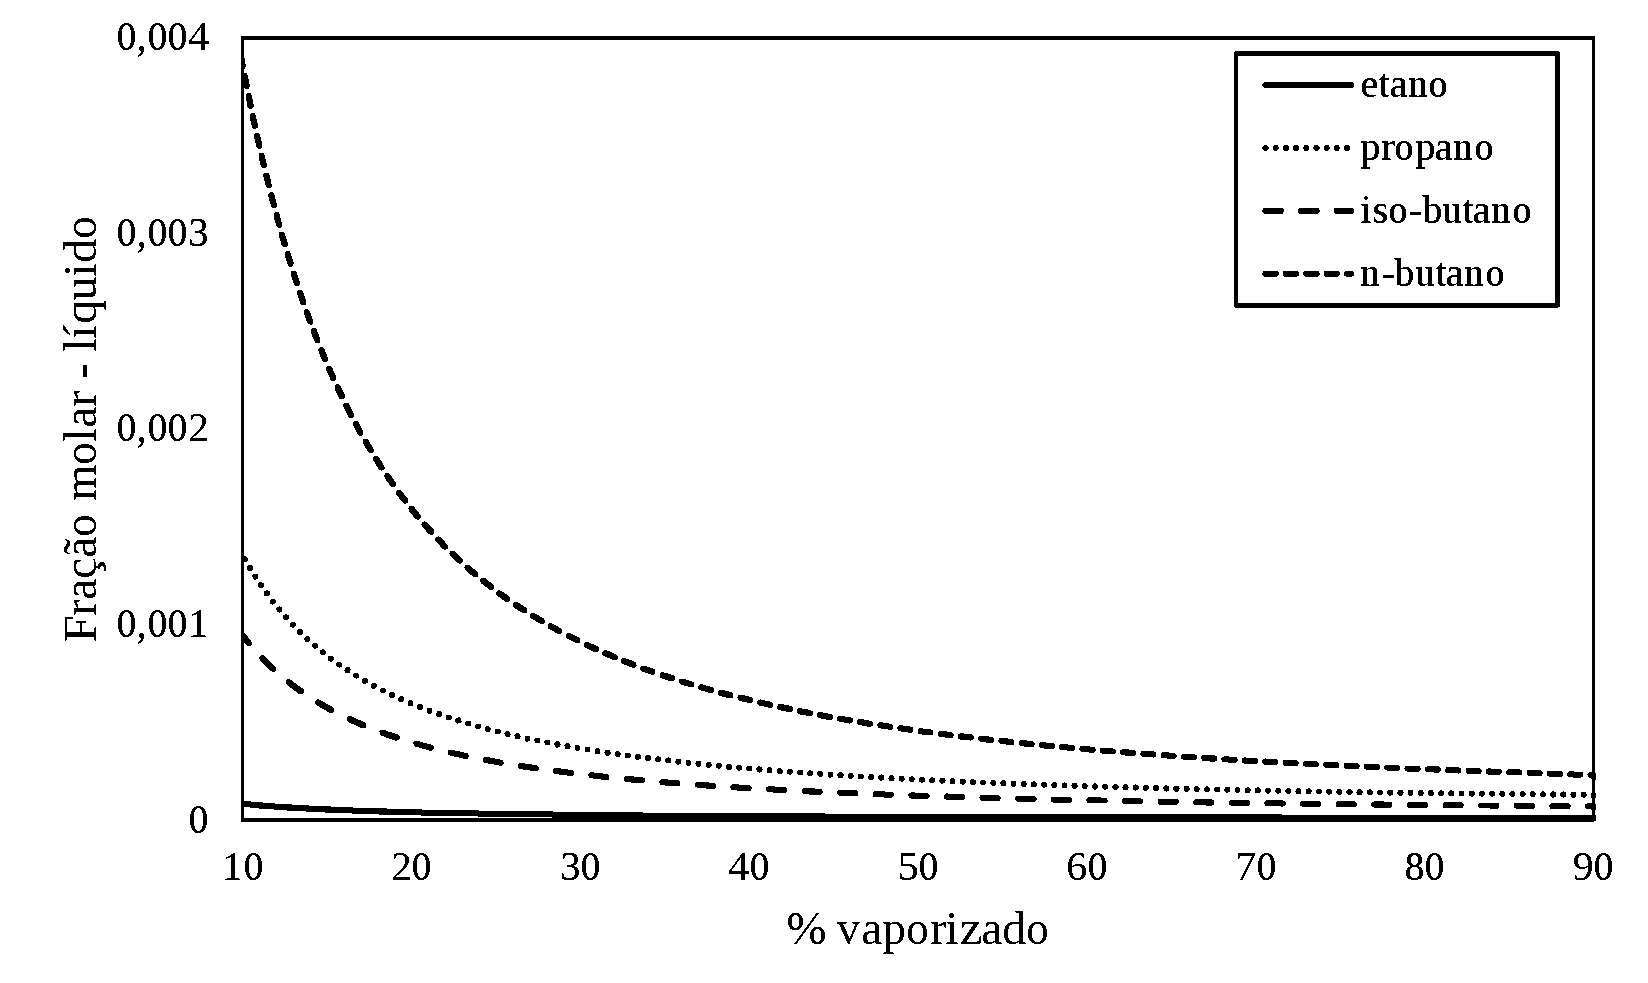
\includegraphics[width=1.0\textwidth]{img/trab3liq.pdf}} 
\caption{Composição dos leves no produto de fundo em função do
percentual vaporizado}
\label{fig:liq}
\end{figure}

A \autoref{fig:liqall} apresenta uma análise da fração molar de alguns pseudo
componentes no fundo do flash. Os componentes foram
selecionados aleatoriamente e a legenda apresenta a massa molar respectiva.
Observa-se que os componentes mais leves são os primeiros a vaporizarem a tenderem sua fração molar à zero. Já os mais pesados apresentam um ponto máximo de fração 
molar antes de também reduzirem.

\begin{figure}[htb] 
\centering
{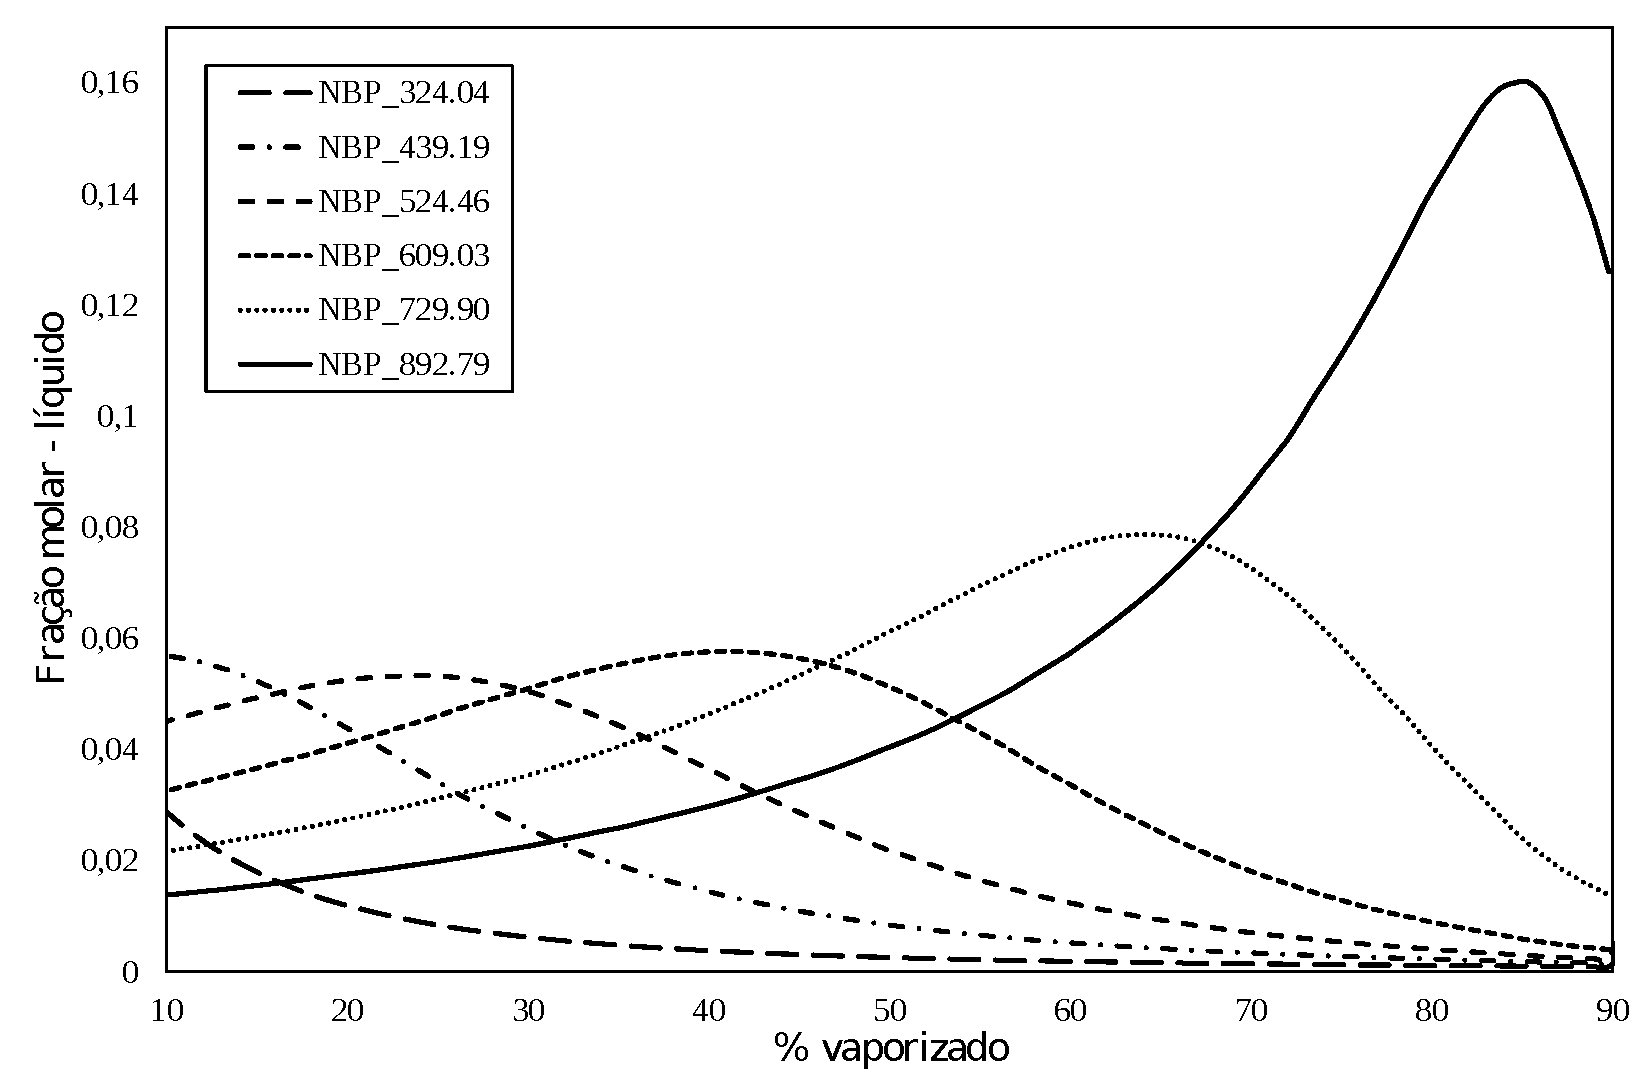
\includegraphics[width=1.0\textwidth]{img/trab3liqall.pdf}} 
\caption{Composição de alguns pseudos no produto de fundo em função do
percentual vaporizado}
\label{fig:liqall}
\end{figure}

A \autoref{fig:vap} mostra a fração molar e o porcentual vaporizado no produto
de topo para os componentes leves (etano, propano, iso-butano e n-butano), em fase vapor. 
Observa-se que todos seguem o mesmo comportamento apresentado na
\autoref{fig:liq}, a exceção de que os valores finais não mais tendem a zero.
Por ser o componente de menor porcentagem volumétrica na alimentação, o etano praticamente não aparece
a partir dos 40{\%} vaporizados. Os demais se apresentam, no final, seguindo a
{\%} ordem de quantidade, em volume, na composição de alimentação, ou seja, 
o n-butano detém a maior fração molar, entre os 4 componentes comparados, 
com cerca de 0,04{\%}.

\clearpage

\begin{figure}[htb]
\centering
{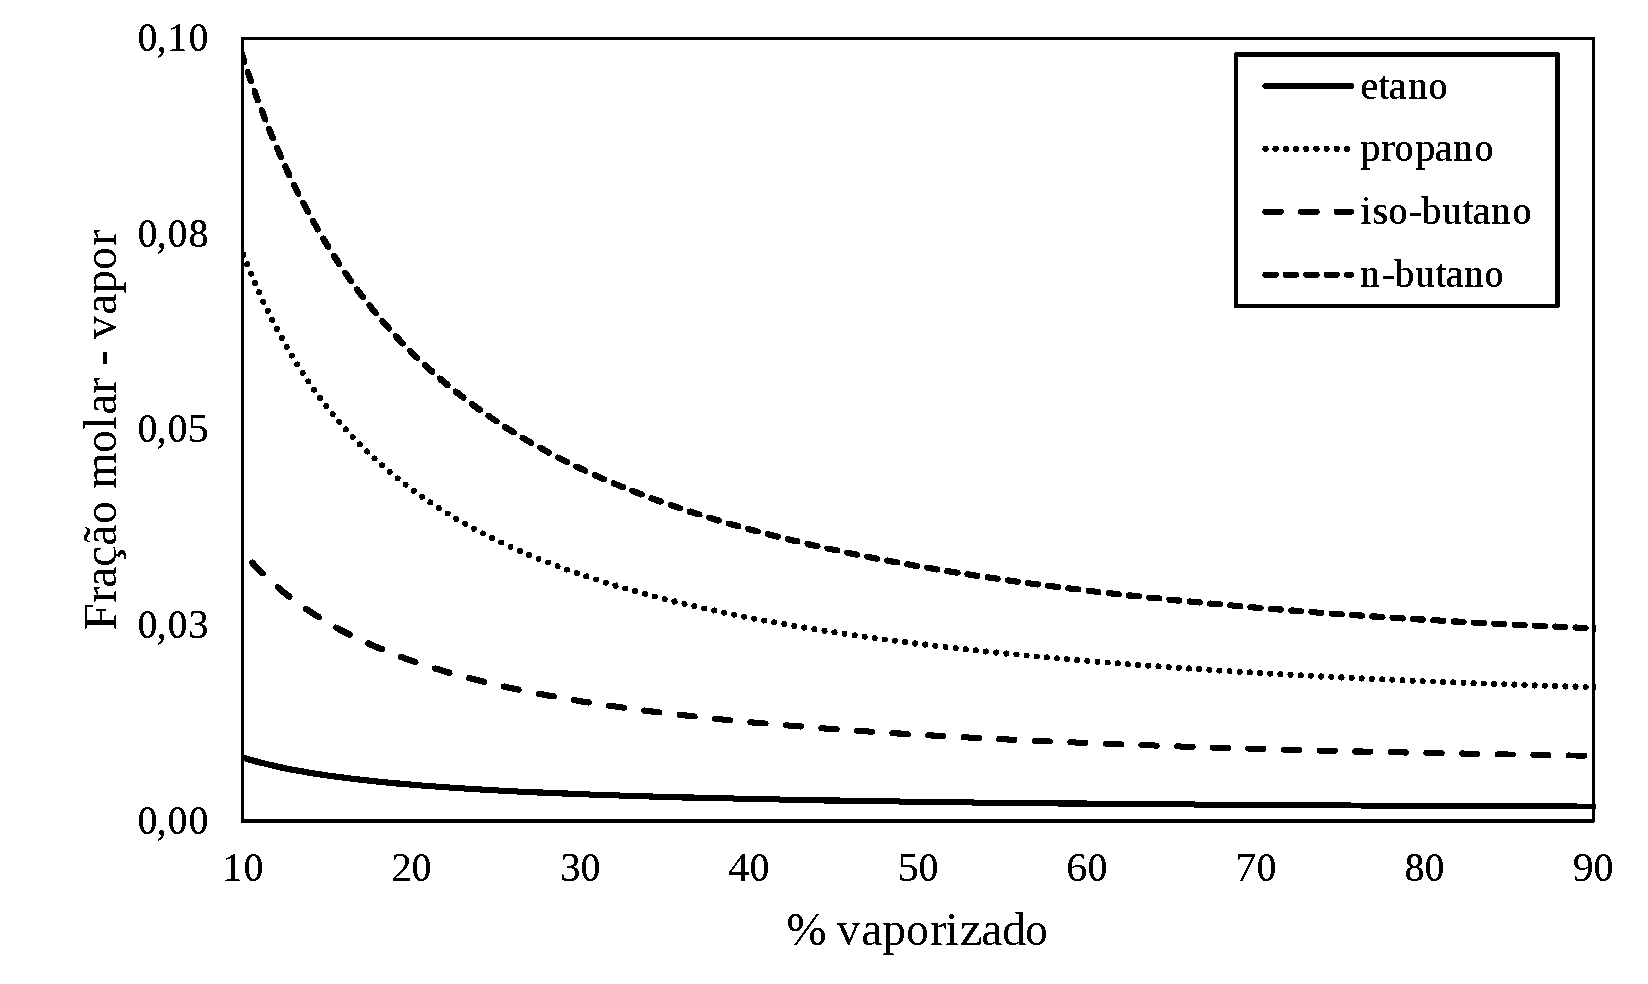
\includegraphics[width=1.0\textwidth]{img/trab3vap.pdf}} 
\caption{Composição dos leves no produto de topo em função do percentual
vaporizado}
\label{fig:vap}
\end{figure}

A \autoref{fig:vapall} evidencia a fração molar em função do porcentual vaporizado
os mesmos componentes pesados mostrados na \autoref{fig:liqall}, mas agora em
fase vapor, no produto de topo. Observa-se que aquele de menor massa molar
apresenta decaimento da sua fração molar devido ao acréscimo das demais. Além disso, como esperado, os 
componentes mais pesados surgem, na figura, ao passo que a vaporização
acontece.

\clearpage

\begin{figure}[htb]
\centering
{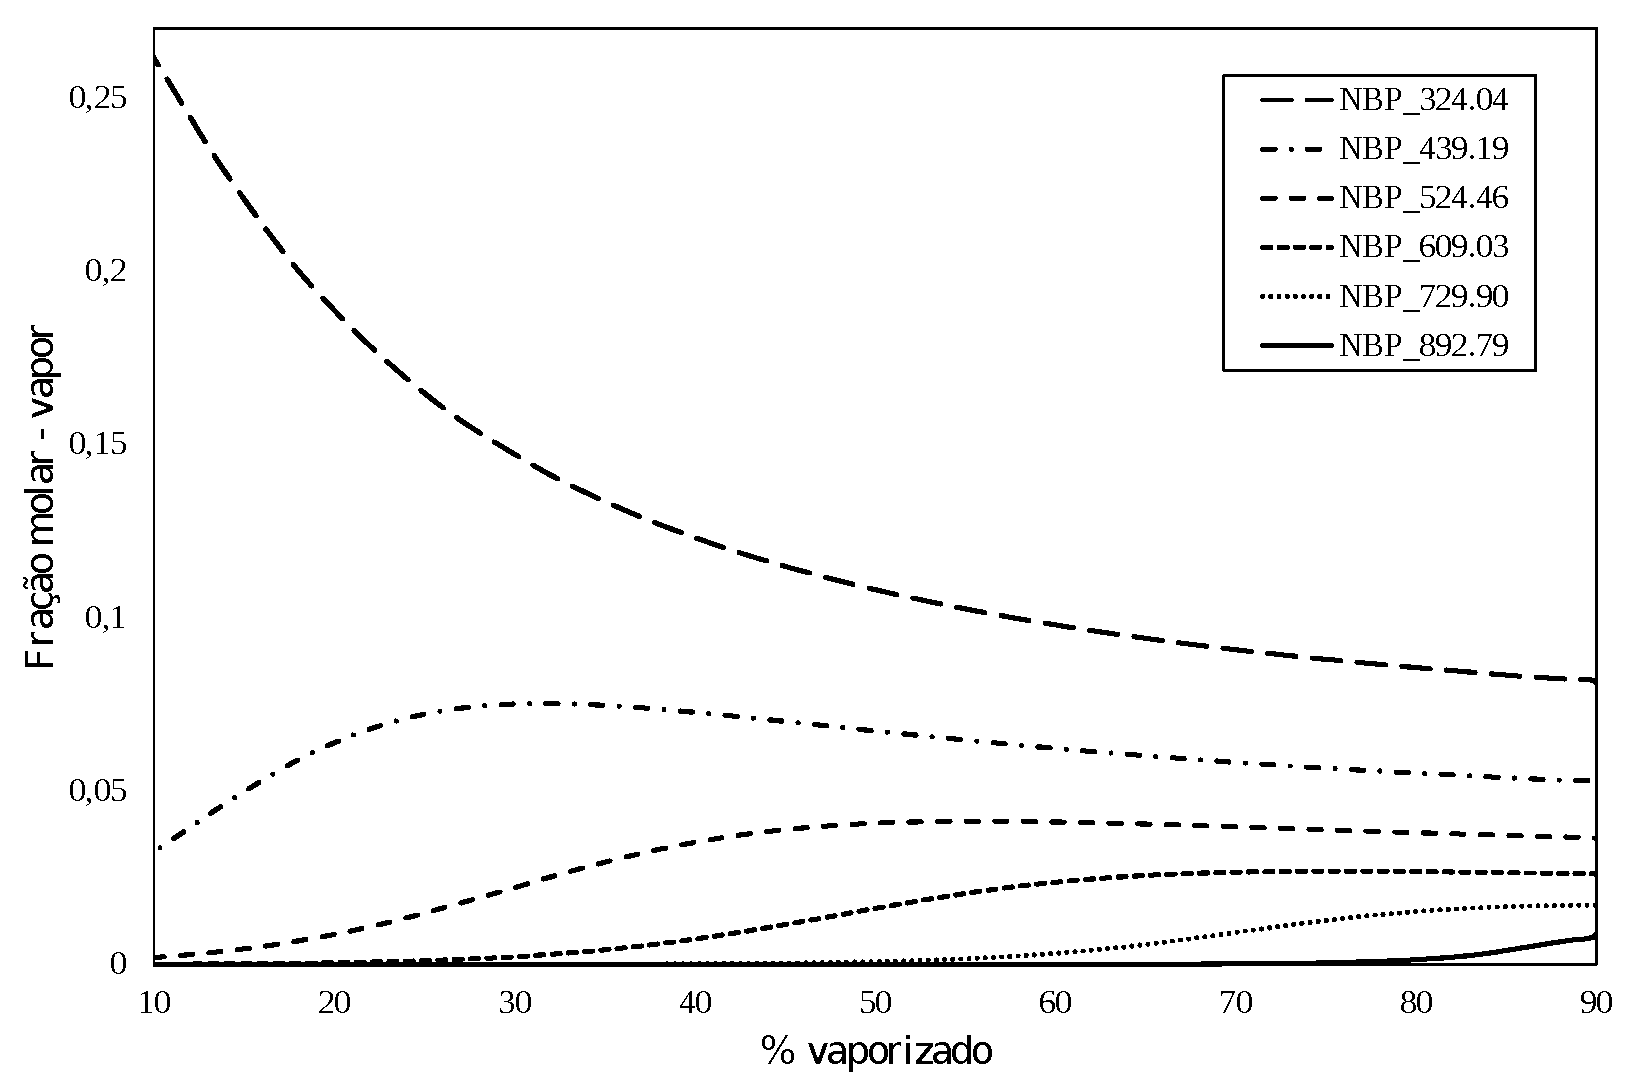
\includegraphics[width=1.0\textwidth]{img/trab3vapall.pdf}} 
\caption{Composição de alguns pseudos no produto de topo em função do
percentual vaporizado}
\label{fig:vapall}
\end{figure}

\clearpage
\section{Conclusões}  

